\documentclass{article}

\usepackage[ngerman]{babel}
\usepackage{pdfpages}
\usepackage{amssymb}
\usepackage{amsmath}
\usepackage{graphics}
\usepackage{graphicx}
\usepackage{geometry}
\usepackage{float}

\geometry{
 a4paper,
 total={170mm,257mm},
 left=25mm,
 top=25mm,
}


\begin{document}

    \title{Praktikum B - Versuch B3.4 Positronen-Emissions-Tomografie}
    \date{\today}
    \author{Jesco Talies, Timon Danowski, Erik Gasmus}
    \maketitle
    \newpage

    \tableofcontents
    \newpage

\section{Einleitung}

PET - Scans geh"oren in der Medizin heutzutage zu den g"angigen Bildgebenden Verfahren. Im Gegensatz zu beispielsweise R"ontgenaufnahmen, CT - oder auch MRT - Scans sind PET -  Scans jedoch nicht sensitiv auf die \textit{Dichte} des untersuchten Gewebes, sondern auf die Konzentration eines zuvor injizierten radioaktiven Markerstoffes, des \textit{Tracers}. Dieser wird durch Ausnutzung der als Begleiterscheinung beim $\beta^+$ - Zerfall auftretenden Positron - Elektron - Annihilation nachgewiesen, bei der zwei Photonen der jeweils spezifischen Energie von 511 keV kollinear emittiert werden. Durch die wiederholte simultane Registrierung zweier solcher Photonen l"asst sich dreidimensional rekonstruieren, wo diese Photonen emittiert wurden, und so die Position der radioaktiven Quelle bestimmen. \\
In diesem Versuch werden wir durch Anwendung dieses Verfahrens versuchen, die Positionen zweier radioaktiver Quellen, die in einer kleinen Box versteckt sind, zu bestimmen. Zudem befassen wir uns mit der Funktionsweise der dazu als Detektor verwendeten NaI - Szintillatoren und der Winkelabh"nagigkeit des Annihilationsprozesses.


\subsection{Theorie}


\subsubsection{Der $\beta$ - Zerfall}


Der $\beta$ - Zerfall ist die am H"aufigsten auftretende Zerfallsart f"ur nat"urlich vorkommende Radionuklide. Man unterscheidet drei Arten des $\beta$ - Zerfalls:

\begin{itemize}
\item{$\beta^-$ - Zerfall:\\
Unter Emission eines Elektrons und eines Antineutrinos kann sich ein Neutron in ein Proton umwandeln:
\begin{equation}
\begin{split}
n &\rightarrow p + e^- + \overline{\nu_e}\\
^A_Z X &\rightarrow ^A_{Z+1}Y + e^- + \overline{\nu}
\end{split}
\end{equation}}
\item{$\beta^+$ - Zerfall:\\
Ebenso kann sich ein Proton durch Emission eines Positrons und eines Neutrinos in ein Neutron umwandeln:
\begin{equation}
\begin{split}
p &\rightarrow n + e^+ + \nu_e\\
^A_Z X &\rightarrow ^A_{Z-1}Y + e^+ + \nu
\end{split}
\end{equation}}
\item{EC (electron capture):\\
Es gibt au"serdem die M"oglichkeit, dass ein Proton durch Einfang eines Elektrons in ein Neutron umgewandelt wird, wobei ein Neutrino emittiert wird:
\begin{equation}
\begin{split}
p + e^- &\rightarrow n + \nu_e\\
^A_Z X + e^- &\rightarrow ^A_{Z-1}Y + \nu
\end{split}
\end{equation}}
\end{itemize}


Nuklide, die zum $\beta^+$ - Zerfall neigen, k"onnen alternativ auch "uber Elektroneneinfang zerfallen. Durch eine genauere Betrachtung der zugeh"origen Energiebilanzen erkennt man, dass das Auftreten der einzelnen Zerfallsarten an folgende Bedingungen gekn"upft ist:

\begin{itemize}
\item{$\beta^-$: $m(^A_Z X) - m(^A_{Z+1}Y) > 0$}
\item{$\beta^+$: $m(^A_Z X) - m(^A_{Z-1}Y) - m_{e^-} - m_{e^+} = m(^A_Z X) - m(^A_{Z-1}Y) - 2m_e > 0$}\footnote{Die Elektronenmasse kommt in die Gleichung, da der Kern nach dem Zerfall ein "ubersch"ussiges Elektron zur Verf"ugung hat, da die Kernladungszahl um 1 sinkt und die H"ullenelektronenzahl sich nicht ver"andert}
\item{EC: $m(^A_Z X) - m(^A_{Z-1}Y) > 0$}
\end{itemize}

Auf der Nuklidkarte findet man $\beta^-$ - Strahler in blau rechts unterhalb der stabilen Isotope (in schwarz), $\beta^+$ - Strahler links oberhalb und in rot.
F"ur die Positron - Emissions - Tomographie ist ausschlie"slich der $\beta^+$ - Zerfall relevant, da nur bei diesem ein Positron entsteht. Die kinetische Energie dieses Positrons variiert, da sich die Zerfallsenergie auf das Positron und das Elektronneutrino verteilt; es wird jedoch schnell durch St"o"se seine kinetische Energie abgeben und dann einen kurzlebigen gebundenen Zustand mit einem Elektron, das \textit{Positronium}, bilden. Dieses zerf"allt, wie eingangs bereits erw"ahnt, unter kollinearer Emission zweier 511 keV - Photonen (\textit{Paarvernichtung}).\\
Da es diese beiden Photonen sind, die beim PET - Scan nachgewiesen werden, ist zu ber"ucksichtigen, dass diese i.d.R. nicht direkt in der Quelle entstehen, sondern eben erst dort, wo das von der Quelle emittierte Positron von einem Elektron eingefangen wird. Dass die Quelle bei einer 3D - Positionsbestimmung m"oglicherweise also leicht verschmiert erscheint, ist durch diesen Umstand bedingt.\\
Beim Zerfall von $^{22}$Na ist zudem zu ber"ucksichtigen, dass es meistens in einen angeregten Zustand von $^{22}$Ne zerf"allt und durch anschlie"sende Emission eines 1275keV-$\gamma$-Quants in den Grundzustand "ubergeht. Das Photon kann, da seine Energie mehr als 1022keV betr"agt, seinerseits in ein Elektron-Positron-Paar zerfallen (sh. Abschn. \textit{Wechselwirkung von $\gamma$-Quanten mit Materie} weiter unten), und das mitunter weit von der Quelle entfernt. Das dabei entstehende Positronium erzeugt bei der darauf folgenden Annihilation mit einem e$^-$ detektierbare Signale au"serhalb der Quelle.




\subsubsection{Paarvernichtung}

Da der Annihilationsprozess f"ur diesen Versuch eine wesentliche Rolle spielt, wollen wir uns noch etwas eingehender mit diesem befassen.\\
Bevor es zur Paarvernichtung kommt, bilden das Positron und Elektron das bereits erw"ahnte Positronium. Der Wirkungsquerschnitt f"ur die Bildung dieses gebundenen Zustands h"angt stark von der kinetischen Energie des Positrons ab: Je schneller das Positron ist, desto unwahrscheinlicher wird der Prozess; daher muss das $e^+$ seine kinetische Energie zuerst abgeben.\\
Sind die Spins im Positronium entgegengesetzt ausgerichtet, spricht man von \textit{Parapositronium}, bei gleich ausgerichteten Spins von \textit{Orthopositronium}. Der zweite Fall tritt nur mit einer Wahrscheinlichkeit von 0,003 \% auf und zerf"allt in insgesamt drei Photonen mit kontinuierlichem Energiespektrum. Die zwei beim Zerfall des Parapositronium emittierten Photonen haben aufgrund der Erhaltung von Impuls und Energie im Ruhesystem des Positroniums stets dieselbe, feste Energie von 511keV und werden stets unter einem Winkel von 180$^{\circ}$ zueinander abgestrahlt. Hat das Positronium jedoch eine kinetische Energie relativ zum Beobachter, so wird zum einen aufgrund relativistischer Effekte der Emissionswinkel aus dem Laborsystem kleiner sein als 180$^{\circ}$:

\begin{equation}
\sphericalangle (\gamma_1, \gamma_2) = |180^{\circ} - \arctan{\frac{p_T}{m_e c}}|
\end{equation},

wobei $p_T$ die transversale Impulskomponente des Positroniums gegen"uber der Emissionsrichtung ist. Zum Anderen sorgt der Dopplereffekt f"ur eine Verschiebung der Photonenenergien, sodass der zugeh"orige Peak im Energiespektrum verbreitert erscheint.



\subsubsection{Wechselwirkung von $\gamma$-Quanten mit Materie}

Man unterscheidet drei Mechanismen der Wechselwirkung zwischen $\gamma$-Quanten und Materie: Der Photoeffekt, die Compton - Streuung und die Paarerzeugung. Die Wirkungsquerschnitte f"ur alle drei Prozesse variieren mit der $\gamma$-Energie $E_{\gamma}$ sowie der Kernladungszahl $Z$ des wechselwirkenden Materials.
Im Folgenden geben wir eine "Ubersicht zu den einzelnen Mechanismen.

\paragraph{Photoeffekt}


Wenn ein $\gamma$ - Quant auf ein Atom trifft, kann es seine Energie an eines der H"ullenelektronen abgeben, indem es von diesem Elektron absorbiert wird. Ionisierungsenergien liegen meist im eV - Bereich, sodass das Elektron durch die Energieaufnahme aus der Atomh"ulle befreit wird. Seine kinetische Energie ist danach gleich der Energie des absorbierten $\gamma$ - Quants abz"uglich der Bindungsenergie; da Letztere jedoch um ein Vielfaches kleiner ist, vernachl"assigen wir diese in folgenden Betrachtungen und sehen die Energie eines solchen Photo - Elektrons als dieselbe Energie des urspr"unglichen Photons an.\\
Der Wirkungsquerschnitt des Photoeffekts ist abh"angig von der Kernladungszahl $Z$ des getroffenen Atoms sowie der Photonenenergie $E_{\gamma}$:

	\begin{equation}
		\sigma \propto Z^5 E^{-3,5}_{\gamma}
	\end{equation}

Bei Photonenenergien bis ca. 100 keV ist der Photoeffekt der am H"aufigsten eintretende Wechselwirkungsprozess zwischen $\gamma$ - Quanten und Materie.


\paragraph{Comtpon - Streuung}

Freie Elektronen k"onnen anders als ihre in Atomen gebundenen Artgenossen nicht die gesamte Energie eines $\gamma$ - Quants aufnehmen. Wie viel Energie sie bei einem Sto"s erhalten, ist abh"angig vom Streuwinkel $\theta$. Der Energie"ubertrag auf das Elektron wird maximal f"ur $180^{\circ}$, also R"uckstreuung des Photons, und ist 0 bei $\theta = 0$. Die "Anderung der Wellenl"ange (und damit der Energie) des Photons beim Sto"s ergibt sich aus der Klein - Nisha Formel zu

	\begin{equation}
		\Delta \lambda = \frac{h}{m_{e}c}(1-\cos{\theta})
		\label{eq:com}
	\end{equation}

F"ur den Wirkungsquerschnitt der Compton - Streuung gilt

	\begin{equation}
		\sigma \propto ZE^{-1}_{\gamma}
	\end{equation}

Ab Photonenenergien von ca. 100 keV wird die Compton - Streuung zur dominierenden Wechselwirkungsform.


\paragraph{Paarerzeugung}

Elektronen und Positronen haben eine Ruhemasse von jeweils 511 keV. Ab einer Photonenenergie von 1022 keV kann es also zur Paarerzeugung kommen, d.h. das $\gamma$ - Quant kann in ein Elektron - Positron - Paar zerfallen. Notwendige Bedingung f"ur diesen Prozess ist neben der genannten Mindestenergie die Anwesenheit eines Atomkerns, der durch Aufnahme des Photonenimpulses als R"ucksto"s die Impulserhaltung gew"ahrleistet. "Ubersteigt die Energie des $\gamma$ - Quants 1022 keV, erhalten die entstehenden Leptonen diese "ubersch"ussige Energie als kinetische Energie.\\
Der Wirkungsquerschnitt der Paarerzeugung nimmt mit der Photonenenergie zu,

	\begin{equation}
		\sigma \propto Z^2 \ln{E_{\gamma}}
	\end{equation}

sodass ab Energien von wenigen MeV (abh"angig von der Kernladungszahl $Z$) die Paarerzeugung den Hauptanteil der Wechselwirkungen zwischen $\gamma$ - Strahlung und Materie ausmacht.


\begin{figure}[H]
	\centering
	%\SetFigLayout{1}{1}
	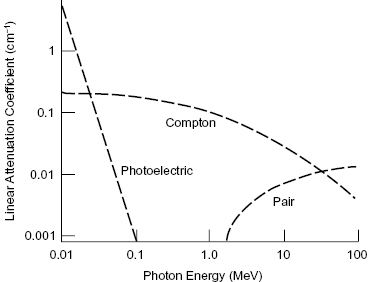
\includegraphics[width=250px, totalheight=250px, keepaspectratio]{WW.PNG}
	%\caption{$\gamma$-Energie vs. Anteile der jew. Wechselwirkungsprozesse \footnote{Quelle: https://sites.google.com/a/umn.edu/mxp/student-projects/2017\_spring/s17\_pairproduction}}
	\label{figWW}
\end{figure}

F"ur die Positron-Emissions-Tomografie ist vor allem die Paarerzeugung relevant, beim Detektionsvorgang spielt jedoch auch der Photoeffekt eine wichtige Rolle, wie der folgende Abschnitt zeigen wird.


\subsubsection{Szintillatoren \& Photomultiplier}

Szintillatoren dienen bei PET zur Umwandlung des initialen, hochenergetischen $\gamma$-Photons in viele einzelne Photonen niedrigerer Energie, deren Gesamtenergie jedoch der des $\gamma$-Quants entspricht. Diese Photonen sto"sen anschlie"send im Photomultiplier mehrere Elektronen heraus, die dort verfielfacht werden, bis sich am Ende ein zur urpr"unglichen $\gamma$-Energie proportionaler, messbarer Strompuls ergibt.

\begin{figure}[H]
	\centering
	%\SetFigLayout{1}{1}
	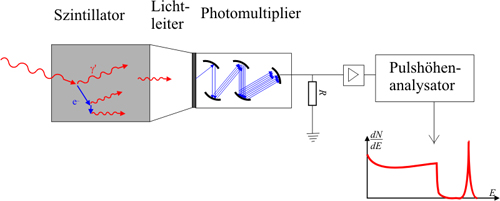
\includegraphics[width=250px, totalheight=250px, keepaspectratio]{Szinti.jpg}
	%\caption{Aufbau Szintillator \& Photomultiplier\footnote{Quelle: http://www.lhc-facts.ch/index.php?page=szintillator, 16.12.2020}}
	\label{figSzinti}
\end{figure}

Trifft das $\gamma$-Photon auf ein H"ullenelektron im Szintillator, nimmt dieses durch den Photoeffekt die gesamte $\gamma$-Energie auf und verl"asst die Atomh"ulle mit entsprechend hoher kinetischer Energie. Im Szintillationskristall wird das e$^-$ nun immer wieder mit Atomen kollidieren und seine Energie st"uckweise an deren H"ullenelektronen abgeben. Diese werden durch die Energieaufnahme in angeregte Zust"ande versetzt und gelangen danach durch Photonenemission in den Grundzustand zur"uck. Auf diese Weise wird das urspr"ungliche Photon in mehrere Photonen niedrigerer Energie umgewandelt.\\
Es gibt verschiedenste Materialien, die sich als Szintillator eignen. Allgemein haben anorganische Szintillationskristalle eine h"ohere Effizienz f"ur den Nachweis von $\gamma$- und R"ontgenstrahlung als organische Szintillatoren, sind daf"ur aber oft hygroskop, was eine luftdichte Lagerung zum Schutz vor Feuchtigkeit unumg"anglich macht (so auch der im Versuch verwendete NaI-Szintillator). Ein wesentlicher Unterschied organischer Szintillatoren zu den anorganischen ist zudem, dass die Szintillation in organischen Materialen durch Elektronen"uberg"ange in Molek"ulen anstelle von "Uberg"angen in Kristallgittern entsteht. Ein organischer Szintillator kann somit auch in fl"ussigem oder gasigem Zustand eingesetzt werden, wogegen anorganische Szintillatoren stets Festk"orper sind.\\
Im Photomultiplier treffen die Photonen zun"achst auf eine Photokathode, aus der sie erneut mittels Photoeffekt Elektronen ausl"osen.
Der Photomultiplier besteht nun aus mehreren ("ublicherweise ungef"ahr 10) \textit{Dynoden}, zwischen denen jeweils ein die Elektronen beschleunigendes Potential liegt. Dadurch l"ost jedes Elektron beim Aufprall auf die jeweils n"achste Dynode ca. $10^7$ weitere Elektronen aus, sodass die resultierende Masse an Elektronen am Ende des Photomultipliers einen messbaren Strom erzeugt.\\
Die Detektion eines einzelnen $\beta^+$-Zerfalls involviert also mehrere Wandlungen zwischen Strahlung und Materie: Zuerst wird beim Zerfall des Radionuklids ein \textit{Positron} und ein Neutrino emittiert. Das Positron zer\textit{strahlt} daraufhin mit einem Elektron und ein \textit{Photon} entsteht. Dieses wird im Szintillator von einem \textit{Elektron} absorbiert, welches mit hoher Geschwindigkeit durch den Szintillator rauscht und bei zahlreichen St"o"sen ebenso zahlreiche �extit{Photonen} erzeugt. Am Photomultiplier werden diese Photonen wieder in \textit{Elektronen} umgesetzt, die anschlie"send verfielfacht werden.





\subsubsection{Durchf"uhrung eines PET - Scans}

Um einen $\beta^+$-Zerfall eindeutig als einen solchen nachzuweisen, gen"ugt es nicht, blo"s eines der emittierten 511keV-Photonen zu registrieren, da wir dieses nicht eindeutig der betrachteten Quelle zuordnen k"onnten. Gelingt es jedoch, \textit{beide} der beim Annihilationsprozess emittierten Photonen \textit{zeitgleich} nachzuweisen, l"asst sich bei einer geeigneten Detektoranordnung sogar die Position der Quelle bestimmen. In der Medizin nutzt man dazu eine ringf"ormige Detektoranordnung wie in Abb.\ref{figPET} dargestellt, die um den Patienten bewegt werden kann; in unserem Versuch ist es g"unstiger, einfach die Quelle zwischen zwei gegen"uber voneinander positionierten Detektoren zu bewegen.

\begin{figure}[H]
	\centering
	%\SetFigLayout{1}{1}
	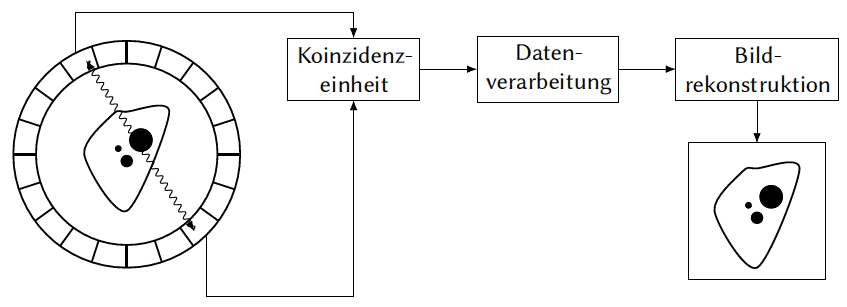
\includegraphics[width=250px, totalheight=250px, keepaspectratio]{PETScanAufbau.PNG}
	\caption[Aufbau PET-Scan]{Aufbau PET-Scan\footnotemark}
	\label{figPET}
\end{figure}
\footnotetext{Quelle: Versuchsanleitung}

Die Detektorelektronik wird so eingestellt, dass sie nur bei der Registrierung von 511keV-Photonen Signale ausgibt, die Koinzidenzeinheit gibt ebenso nur dann Signale aus, wenn beide Detektoren zeitgleich ansprechen. Aus einer gen"ugend gro"sen Menge registrierter Ereignisse l"asst sich dann schlie"slich die Quellenposition rekonstruieren. Dabei k"onnen verschiedene Komplikationen die Bildqualit"at negativ beeinflussen: Die beim $\beta^+$-Zerfall emittierten Positronen haben eine Reichweite von ca. 2mm, wodurch die Bildsch"arfe begrenzt ist und auch \textit{falsche} Koinzidenzen haben einen negativen Einfluss. So k"onnen Photonen \textit{absorbiert} werden, bevor sie den Detektor erreichen, sodass dieser kein Ereignis registriert; es kann durch \textit{Streuung} auf dem Weg zum Detektor Energie verlieren und so die Schwellwertenergie unterschreiten oder es wird durch Streuung abgelenkt und wird an anderer Stelle registriert, woraus sich eine falsche Line of Response erg"abe. Ebenso k"onnen sich zuf"allig auftretende Koinzidenzen (z.B. verursacht durch Untergrundstrahlung) oder Koinzidenzen, die aufgrund nicht erf"ullter Kriterien \textit{verworfen} werden, aber dennoch von der gesuchten Quelle stammen, die Bildqualit"at verschlechtern.\\
Die meisten medizinischen bildgebenden Verfahren sind sensitiv auf die Dichte des untersuchten Gewebes; so absorbieren beispielsweise Knochen oder Metall mehr R"ontgenstrahlung als Fett- oder Muskelgewebe\footnote{R"ontgenstrahlung eignet sich sowohl f"ur 2D - Aufnahmen beim klassischen \textit{R"ontgen} oder auch f"ur 3D - Aufnahmen oder 2D - Querschnitte mittels Computertomografie}, Ultraschallwellen breiten sich in unterschiedlich dichtem Gewebe mit unterschiedlicher Geschwindigkeit aus und bei einer Magnetresonanztomografie werden zun"achst die Protonenspins im K"orper mithilfe eines starken externen Magnetfeldes gleich ausgerichtet und im Anschluss mit einem Radiopuls aus der Ordnung gebracht; die Zeit, bis die Spins sich daraufhin wieder entlang des Magnetfelds ausrichten, ist wiederum charakteristisch f"ur die jeweilige Gewebeart. Mit Ausnahme der Ultraschalluntersuchung belasten all diese Verfahren den K"orper mit unterschiedlich hohen Strahlendosen vom ca. 2-fachen der t"aglichen, nat"urlichen Untergrundstrahlung bei R"ontgenaufnahmen des Brustkorbbereiches bishin zum 1000-fachem davon bei CT-Scans des Abdominalbereichs.  Keines dieser Verfahren ist au"serdem geeignet, um z.B. Krebszellen im K"orper zu lokalisieren, da diese sich hinsichtlich ihrer Dichte nicht vom umgebenden Gewebe unterscheiden. Ein wesentlicher Unterschied zwischen Krebszellen und gesunden Zellen ist jedoch ihre deutlich erh"ohte Reproduktionsrate.\\
K"orperzellen ben"otigen Glucose zur vermehrung, ein Stoff der sich mit Fluor markieren l"asst; verwendet man dazu das radioaktive Isotop $^{18}$F und injiziert diesen \textit{Tracer} einem Patienten, wird er sich also vermehrt in Krebszellen ansammeln. Da es sich bei $^{18}$F zudem um einen $\beta^+$-Strahler handelt, l"asst sich auf diese Weise mittels PET die Position der Krebszellen im K"orper dar"uber bestimmen, dass diese mehr $\beta$-Strahlung als das restliche Gewebe emittieren und sich so im PET-Scan von diesem abheben.\\
Nicht jeder $\beta^+$-Strahler eignet sich als Tracer, denn zum Einen kann der menschliche K"orper nicht jedes Element gefahrlos verarbeiten, zum Anderen sollte der K"orper auch nicht "uber lange Zeit durch Strahlung von innen heraus belastet werden. Ein Tracer sollte also sowohl eine niedrige Halbwertszeit $T_{1/2}$ aufweisen, damit dieser sich schnell wieder aus dem K"orper verfl"uchtigt, und au"serdem sollte das Element in K"orpereigenen Verbindungen vorhanden sein, um den K"orper nicht noch mit der Verarbeitung des Stoffes zu strapazieren. Besonders geeignet sind daher z.B. 20,3 min $^{11}$C ($T_{1/2}=20,3$min), $^{13}$N ($T_{1/2}=10,1$ min), 2,03 min $^{15}$O ($T_{1/2}=2,03$ min) oder eben $^{18}$F ($T_{1/2}=110$min). Durch die niedrigen Halbwertszeiten der Isotope ist es unerl"asslich, diese direkt vor Ort der PET-Anlage zu produzieren, was mit hohen Kosten in der Anschaffung sowohl des PET-Scanners als auch eines geeigneten Teilchenbeschleunigers zur Radionuklidherstellung (z.B. ein Zyklotron) sowie hohen laufenden Kosten aufgrund des Energiebedarfs verbunden ist.





\subsubsection{Detektorelektronik}


\begin{figure}[H]
	\centering
	´%\SetFigLayout{1}{1}
	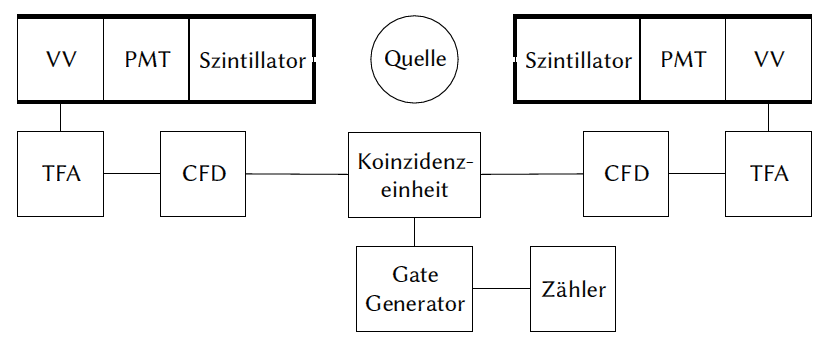
\includegraphics[width=250px, totalheight=250px, keepaspectratio]{elektronik.PNG}
	\caption[Schaltskizze der verwendeten Elektronik]{Schaltskizze der verwendeten Elektronik\footnotemark}
	\label{figElektronik}
\end{figure}
\footnotetext{PMT: Photomultiplier, VV: Vorverst"arker, TFA: Timing Filter Amplifier (Hauptverst"arker), CFD: Constant Fraction Discriminator. Quelle: Versuchsanleitung}

Das elektrische Signal, das bei einem Ereignis am Ende des \textit{Photomultipliers} (kurz: PMT) abgegriffen werden kann, muss zur Umsetzung des im letzten Abschnitt beschriebenen Verfahrens durch einige elektronische Bauteile verarbeitet werden (sh. Abb. \ref{figElektronik}), mit deren Aufgaben wir uns im Folgenden befassen.\\
Zun"achst wird die Amplitude des abgegriffenen Signals durch einen \textit{Vorverst"arker} (=VV) erh"oht, sodass die Bauteilbedingten Verluste (Eigenwiderst"ande der Kabel, Schnittstellen usw.) gering gehalten werden. Der anschlie"sende \textit{Hauptverst"arker}, ein \textit{Timing Filter Amplifier}, dient dazu, als Reaktion auf ein eingehendes Signal ein Signal mit m"oglichst steiler Anstiegsflanke auszugeben, damit die Reaktionszeit des gesamten Detektors niedrig bleibt und wir kurz aufeinander folgende Koinzidenzen gut voneinander Trennen und als einzelne Ereignisse erfassen k"onnen.\\
Darauf folgt der\textit{Constant Fraction Discriminator} (=CFD), der ein logisches Signal ausgibt, wenn sein Eingangssignal einen gewissen Schwellwert "ubersteigt. Die dahinter geschaltete Koinzidenzeinheit erh"alt also von beiden CFDs logische Signale und gibt ihrerseits genau dann ein logisches Signal aus, wenn die von den CFDs erhaltenen Signale zeitlich "uberlappen. Dabei kann es passieren, dass zwei Signale, die zwar koinzident sind, aber unterschiedliche Amplituden haben, den Schwellwert im Diskriminator zu verschiedenen Zeiten "uberschreiten (\textit{Walk}-Effekt, sh. Abb. \ref{figWalkDerHurensohn}), oder aber zwei identische Signale durch "Uberlagerungen mit dem Untergrund im zeitlichen Verlauf voneinander abweichen und die beiden Diskriminatoren zu unterschiedlichen Zeiten die logischen Antwortsignale ausgeben (\textit{Jitter}-Effekt). Diesen beiden Effekten beugt der CFD vor, indem er das Eingangssignal um eine kurze Zeit $T$ verz"ogert und diesem ein zweites Signal "uberlagert, das aus dem Eingangssignal durch Inversion und Stauchung um einen Faktor $0<k<1$ erzeugt wird (sh. Abb. \ref{figCFD}). Der Nulldurchgang dieses manipulierten Signals ist unabh"angig von der Pulsh"ohe des Eingangssignals (sh. Abb. \ref{figWalkDerHurensohn}) und somit gibt der CFD ein logisches Signal bei diesem Nulldurchgang aus und minimiert dadurch Walk- und Jitter-Effekt.


\begin{figure}[H]
	\centering
	%\SetFigLayout{1}{1}
	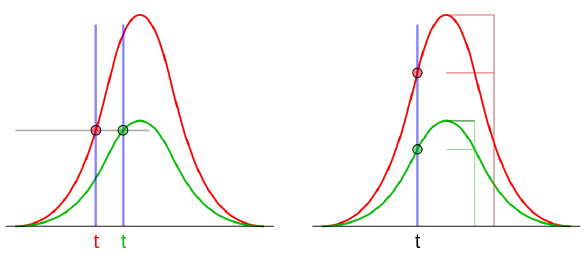
\includegraphics[width=250px, totalheight=250px, keepaspectratio]{Walk.PNG}
	\caption[Walk-Effekt; Links: Schwellendiskriminator, Rechts: CFD]{Walk-Effekt; Links: Schwellendiskriminator, Rechts: CFD\footnotemark}
	\label{figWalkDerHurensohn}
\end{figure}
\footnotetext{Quelle: Versuchsanleitung}

\begin{figure}[H]
	\centering
	%\SetFigLayout{1}{1}
	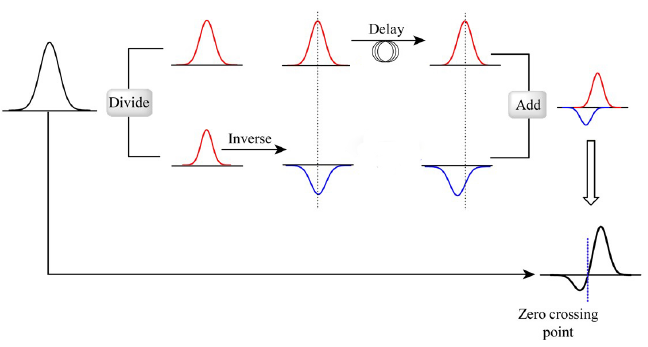
\includegraphics[width=250px, totalheight=250px, keepaspectratio]{CFD.PNG}
	\caption[Funktionsweise eines CFD]{Funktionsweise eines CFD\footnotemark}
	\label{figCFD}
\end{figure}
\footnotetext{Quelle: Versuchsanleitung}

Das logische Signal, welches die Koinzidenzeinheit bei einem zeitlichen "Uberlapp der von den CFDs erhaltenen Signale ausgibt, wird zuletzt noch mithilfe eines \textit{Gate Generators} in ein genormtes logisches Signal gewandelt, damit der Z"ahler dieses verarbeiten kann. Der Z"ahler selbst z"ahlt schlicht die Menge der erhaltenen Signale in einem vorgegebenen (einstellbaren) Zeitraum.



    \section{Versuchsdurchführung}
        Messaufträge:
        \begin{enumerate}
            \item Vorverstärkersignal am Oszilloskop. Detektoren and Hochspannung anschließen, Quelle in der Mitte der Detektorfläche platzieren. Signal skizzieren.
            \item TFAs einbauen und das Gaussignal am Oszilloskop betrachten
            \item CDDs einbauen und die Nulldurchgänge am Oszilloskop untersuchen, verschiedene einstellungen des CFD testen, Einfluss auf die Zählrate beobachten
            \item Ortsauflösung bestimmen, Lage der quelle bezüglich der Line of Response ändern, dazu Quelle auf wagen legen, wagen mit fester Schrittweite verschieben
            im vom Detektor abgedeckten Bereich, Anzahl der Koinzidenzen in 60s Messbereich messen, insgesamt 20 Messwerte
            \item Messen der Zählraten auf X Achse -> Y Achse und dann diagonal
            \item Winkelabhängigkeit: CFD so einstellen das nur die 511 keV Linien betrachtet werden, Winkelbereich -5° - 5° in 0.5° schritten messen.
            Danach 511keV auf dem 1ten Detektor messen und 1275 keV linie auf dem 2ten Detektor messen. Aufgrund der mittleren Lebensdauer von 22Ne von 4ps und der
            hohen Wahrscheinlichkeit eines angeregten Kerns ist wahrscheinlich keine signifikante Reduktion der Zählrate zu erwarten
        \end{enumerate}
    \section{Messwerte}

    \section{Auswertung}
        \begin{itemize}
            \item Höheres Signal 1275er linie, niedrigeres 511keV
            \item Signalhöhe -> Signalstärke/Energie, Signalbreite -> TFA bedingt / FWHM
            \item TFA -> Gausskurve -> CFD Nulldurchgänge -> Coincidence Counter Logic1/0
            \item
        \end{itemize}

        \subsection{Signale Am Oszilloskop}
            Im ersten Abschnitt der Auswertung befassen wir uns mit der Signalverarbeitung und den verschiedenen
            Schritten, in dem wir die verschiedenen Ausgangssignale der elektronischen Signalverarbeiter am Oszilloskop betrachten.


            \subsubsection{Szintillator und Vorverstärker}
                Folgende Graphik zeigt das Signal direkt nach der Szintillatorschaltung, bestehend aus
                dem Szintillator selbst, dem Photomultiplier und dem Vorverstärker.
                \begin{figure}[H]
                    \centering
                    \includegraphics{Images/SzintillatorSignal.JPG}
                    \caption{Szintillator Signal}
                \end{figure}
                Obwohl man nach physikalisch ein Negativen Spannungsimpuls erwarten würde ist dieses Signal jedoch Positiv, dies ist für die
                Messung jedoch vollkommen unerheblich und ist lediglich durch die Wahl der Vorverstärkers bestimmt.
                Die Höhe des Peaks (hier ca. $390mV$) ist dabei direkt proportional zur Energie des gemessenen
                Ereignisses. Die Breite des Peaks (hier ca $200\mu s$) entsteht hierbei hauptsächlich durch das entladen von Kapazitäten
                welche im Vorverstärker verbaut sind.

            \subsubsection{Timing Filter Amplifier}
                Das folgende Signal ist der Ausgang des TFA bei Eingang des obigen Signals der Szintillatorschaltung.
                \begin{figure}[H]
                    \centering
                    \includegraphics{Images/TFASignal.JPG}
                    \caption{TFA Singal}
                \end{figure}
                Auch hier fällt direkt auf, das die Polarität des Spannungsimpulses gewechselt hat, auch dies ist für die Auswertung irrelevant und
                nur durch die Wahl des TFA bestimmt. \newline
                Das Signal wird durch den TFA in seinem Informationsgehalt kaum beeinflusst, er dient lediglich der Aufbereitung für
                die Verarbeitung durch den CFD. Die Höhe des Peaks (hier ca. $4,85V$) und Breite des Signals (hier ca $1s$) tragen dabei die selben
                Informationen.

            \subsubsection{Constant Fraction Discriminator}
                Nun kommen wir zum ersten auswertenden Element, die folgende Signale sind sowohl der Analoge- als auch der Digitale des CFD.
                \begin{figure}[H]
                    \centering
                    \includegraphics{Images/CFDSignal.JPG}
                    \caption{CFD Signal, Analog(Gelb) Digital(Blau)}
                \end{figure}
                Das analoge Signal trägt nun nicht länger unsere Informationen, es dient an dieser stelle lediglich der Veranschaulichung des
                Prinzips des CFD, da man deutlich erkennt, das dieser bei Nulldurchgang des Verarbeiteten Signals ein Logisches Signal
                von ~0.8V bzw. Logisch 1 emittiert, welches für ~1s bestehen bleibt. Die Signalhöhe ist dabei eigentlich egal, da uns hierbei nur
                dessen Logisches Äquivalent interessiert, die Signalzeit hingegen ist äußerst interessant, da diese unseren Toleranzbereich definiert
                indem 2 Logische Signale noch als Koinzidenz anzusehen sind. Welche Signale überhaupt einen Logischen Output erzeugen lässt sich über
                die Obere- und Untere Schwelle einstellen, durch die Signale mit Höhen unter oder Über den Grenzwerten verworfen werden. Diese Einstellungen
                sind notwendig um sowohl schwaches Hintergrundrauschen unterhalb der unteren schwelle zu verwerfen, als auch die 1275keV Linie zu verwerfen,
                da für die Gewünschten Zählraten nur Teilchen mit Energien um 511keV gemessen werden sollen.

                \subsubsection{Zusammenfassung}
                Um den oben Dargestellten Prozess noch einmal kompakt zusammenzufassen:
                \begin{itemize}
                    \item Der Szintillator liefert einen Peak proportional zur Teilchenenergie des Detektierten Teilchens
                    \item Im TFA wird das Signal weiter aufbereitet und Verstärkt
                    \item Der CFD Bestimmt ob es sich um einen zulässigen Peak handelt und emittiert ein entsprechendes Logisches Signal
                \end{itemize}

        \subsection{Bestimmung der Ortsauflösung}
            Um nun die Ortsauflösung unseres Aufbaus zu bestimmen wurde die Anzahl der detektierten Ereignisse in 60 Sekunden
            für verschiedene Verschiebungen der Quelle relativ zum Aufbau aufgetragen. Die daraus resultierende Verteilung wird gut genähert durch eine
            Gaußkurve wie im folgenden Bild dargestellt wird:
            \begin{figure}[H]
                \centering
                \includegraphics[width=0.9\textwidth]{Ortsauflösung.png}
                \label{Plot der Ortsauflösungsmessung}
            \end{figure}
            Aus dem Fit geht eine Halbwertsbreite von $FWHM=(2,8\pm0,11)mm$ hervor, diese Breite dient uns für die folgende Versuchsteile als 
            Messkopfbreite bzw. als Ortsfehler, da in diesem Bereich kaum Verluste der Messrate festzustellen sind auch wenn die Probe nicht ideal
            zentriert ist. In diese Messung fließt jedoch zunächst zusätzlich noch die Ungenauigkeit der Positionsbestimmung ein, bei der wir den Wagen
            mit etwas Schlupf in 1mm Schritten bewegen konnten. Halbmillimetrige Messwerte sind dabei nur schwer einzustellen wodurch wir einen Fehler von
            etwa 1mm annehmen.


        \subsection{Auswertung des PET-Scans}
            In diesem Abschnitt des Versuchs wurde ein PET-Scan simuliert über 2 in einer Truhe verschlossenen Quellen deren Positionen ohne diese zu sehen
            bestimmt werden sollten. Dafür haben wir durch Wiederholung der Ortsauflösungsmessung in X, Y und Diagonalrichtung folgende Tabelle erstellen können:
            \begin{figure}[H]
                \centering
                \includegraphics[width=0.9\textwidth]{xy-messung.pdf}
                \label{Tabelle der Messungen in X und Y Richtung}
            \end{figure}
            \begin{figure}[H]
                \centering
                \includegraphics[width=0.9\textwidth]{diag-messung.pdf}
                \label{Tabelle der Messungen in Diagonalrichtung}
            \end{figure}
            \begin{figure}[H]
                \centering
                \includegraphics[width=0.9\textwidth]{finalverdict.pdf}
                \label{Überlagerung beider Messungen und Position der Quellen}
            \end{figure}
            \begin{figure}[H]
                \centering
                \includegraphics[width=0.7\textwidth]{PET-scanReal.jpg}
                \label{Tatsächliche Position der Quellen}
            \end{figure}
            Diese Vorgehensweise gibt uns letztendlich recht präzise Kentniss über die Position unserer Quellen.



        \subsection{Analyse der Winkelabhängigkeit}
            Im letzten Schritt soll nun noch die Winkelabhängigkeit unseres Scanners bestimmt werden, dazu wurde zunächst die Koinzidenzzählrate
            der 511/511 Linien unter veränderten Einfallswinkeln gemessen und danach die der 1275/511 Linien und selbigen Winkeln.
            \begin{figure}[H]
                \centering
                \includegraphics[width=0.7\textwidth]{Winkelauflösung.png}
                \label{Winkelauflösung}
            \end{figure}
            Dabei sieht man zunächst die wie bei der Ortsauflösung bereits gemessene Gaussähnlichkeit der 511/511 Linie wohingegen die 
            Koinzidenz der 511/1275 keinerlei vorhersagbares Verhalten aufweist. Zudem kann man dem Fit der Gaußkurve auch hier eine 
            Art Messkopf-Winkelauflösung entnehmen, die der Halbwertsbreite des Fits entspricht, diese ist etwa $$FMWH=(3,38\pm 0,14)°$$
            Die starke Winkelabhängigkeit ist ein großer Vorteil bei der PET als bildgebende Methode, da die LoR dadurch mit großer Genauigkeit
            ermittelt werden kann.
            
    \section{Diskussion}

\end{document}